\documentclass[conference]{IEEEtran}
\IEEEoverridecommandlockouts
% The preceding line is only needed to identify funding in the first footnote. If that is unneeded, please comment it out.
\usepackage{cite}
\usepackage{amsmath,amssymb,amsfonts}
\usepackage[ruled,vlined,linesnumbered]{algorithm2e}
\usepackage{graphicx}
\usepackage{textcomp}
\usepackage{xcolor}
\usepackage[hidelinks]{hyperref}
\usepackage{float}
\usepackage{booktabs}
\usepackage{pgfplots}
\usepackage{tikz}
\usetikzlibrary{positioning,calc,arrows.meta,shapes.geometric,fit,backgrounds}
\usepackage{placeins}
\pgfplotsset{compat=1.18}
\newcommand{\missing}[1]{\textit{#1}}
\def\BibTeX{{\rm B\kern-.05em{\sc i\kern-.025em b}\kern-.08em
    T\kern-.1667em\lower.7ex\hbox{E}\kern-.125emX}}
\begin{document}


\title{
\fontsize{22}{25}\selectfont
CodeSheriff: Design and Development of an Agentic Security
Auditor for an SFI-Enabled Confidential CI/CD Execution
Layer Using Bayesian Vulnerability Inference
}

\author{\IEEEauthorblockN{Shubhankar Vishnu Patil}
\IEEEauthorblockA{\textit{Dept. of Information Technology} \\
\textit{G H Raisoni College of Engineering and Management}\\
Pune, India \\
shubhankarp258@gmail.com}
\and
\IEEEauthorblockN{Vivek Dnyaneshwar Joshi}
\IEEEauthorblockA{\textit{Dept. of Information Technology} \\
\textit{G H Raisoni College of Engineering and Management}\\
Pune, India \\
vivekdjoshi05@gmail.com}
\and
\IEEEauthorblockN{Yash Suresh Kodgirwar}
\IEEEauthorblockA{\textit{Dept. of Information Technology} \\
\textit{G H Raisoni College of Engineering and Management}\\
Pune, India \\
yashkodgirwar@gmail.com}
\and
\IEEEauthorblockN{Nirmalya Mukhopadhyay}
\IEEEauthorblockA{\textit{Dept. of Information Technology} \\
\textit{G H Raisoni College of Engineering and Management}\\
Pune, India \\
}
\and
\IEEEauthorblockN{Kunal Kundu}
\IEEEauthorblockA{\textit{Dept. of Information Technology} \\
\textit{G H Raisoni College of Engineering and Management}\\
Pune, India \\
}
}

\maketitle

\begin{abstract}
Modern software development increasingly relies
on Continuous Integration/Continuous Deployment (CI/CD) pipelines to deliver software rapidly, but automated
security review at the pull request stage remains limited. Existing
security tools rely on rigid static analysis or homogeneous multi-
agent approaches, which may generate false positives or overlook
complex vulnerabilities. This project will present CodeSheriff, an
agentic security auditor that will analyze GitHub pull requests
using structural, semantic, contextual, and SFI-based confidential
execution analysis. A Bayesian inference engine will fuse evidence
from multiple agents to generate confidence-aware vulnerability
assessments, while an automated patch generation and verifica-
tion module will recommend and validate fixes through GitHub
and a web dashboard. The system will enhance CI/CD security
by delivering reliable, explainable, and statistically grounded
vulnerability detection while reducing manual review effort.
\end{abstract}
\vspace{6pt}
% \begin{IEEEkeywords}
%  Vulnerability Detection, Multi-Agent Systems, Bayesian Inference, CI/CD , Software Fault Isolation(SFI)
% \end{IEEEkeywords}
\begin{IEEEkeywords}
vulnerability detection, multi-agent systems, software security,
continuous integration and continuous deployment, 

\end{IEEEkeywords}


\section{Introduction}
In today’s software industry, developers frequently push code to the main branch through Pull Requests (PRs). However, security analysis of each Pull Request is still largely performed manually, making the review process more time-consuming.Teams either use basic approaches that only catch known, simple mistakes, or they don't have enough time to properly review every pull request. This is a big problem because even one missed vulnerability can put the whole application at risk once the code is merged and deployed. On top of this, attackers are now also targeting the Continuous Integration/Continuous Deployment (CI/CD) that's builds and runs the code.

Solutions that exist today don’t fully solve this problem. Traditional static analysis approaches identify fixed patterns but are unable to catch tricky ones, so they generate a lot of false alarms. Some recent tools use multiple artificial intelligence (AI) agents, but all these agents basically read the same code in the same way, so they don't really give different opinions. when these approaches combine results, they just use simple voting, which doesn't tell you how confident the final answer actually is.

In this paper, we are proposing CodeSheriff to fix this problem. It uses four different types of agents that look at the code from different perspectives. Static agent checks the code structure, the meaning of the code is understood by the semantic agent, the context agent checks whether accepting this PR could bring back any vulnerability from previously accepted PR, and the runtime agent actually watches the code run inside a safe, isolated environment using software fault isolation (SFI). All this information is then combined using a Bayesian model, which gives a clear probability of whether the code is vulnerable, along with how confident the system is. This same safe environment also protects the CI/CD workflow, since it only releases secret keys when it is sure the correct, verified code is running.


The rest of this paper is structured as follows. Section \ref{LS} talks about related work already done in this area. Section \ref{PS} explains our proposed method and how the system is designed.

\section{Literature Survey} \label{LS}

Early learning-based studies explored structural and sequential representations for vulnerability detection. Li and Yang \cite{ref20} compared sequence and graph-based deep learning methods, identifying challenges in capturing long-range dependencies and generalizing to noisy data. CODE-SMASH \cite{ref19} and XTransformer \cite{ref18} employed hierarchical neural and transformer architectures to capture multi-level code representations and improve similarity-based detection, while remaining sensitive to computational cost and dataset characteristics . Abbasi and Shameli-Sendi \cite{ref4} used Code Property Graph metrics with machine learning for interpretable vulnerability and vulnerability-type prediction, but their approach was limited to C/C++. DeepSecure \cite{ref2} combined CodeBERT with bidirectional long short-term memory(BiLSTM) and convolutional neural network(CNN) layers for python vulnerability detection, incorporating robustness and confidence calibration, but remained language-specific and affected by noisy labels.

Transformer and large language model(LLM) based approaches have subsequently improved semantic analysis of source code. Shestov \textit{et al.} \cite{ref13} fine-tuned WizardCoder using parameter-efficient learning for vulnerability classification, but remained limited to function-level analysis. Tamberg and Bahsi and Gnieciak and Szandala \cite{ref14,ref17} benchmarked LLMs against vulnerability detection tasks and traditional static analysis tools, showing strong potential but persistent false positives, hallucinations, localization errors, and inference costs. Gülmez \cite{ref7} surveyed code-generation LLMs and highlighted challenges in structural correctness, repository-level reasoning, and security. Chen \textit{et al.} \cite{ref9} and Su \textit{et al.} \cite{ref8} similarly identified limitations involving context windows, hallucination, dataset quality, generalization, and interpretability. Germano \textit{et al.} \cite{ref10} reviewed LLM-based vulnerability detection, repair, and explanation, noting that research remains more focused on detection than automated repair and explanation.

To address the limitations of isolated code analysis, recent studies have incorporated contextual and repository-level information. Antal \textit{et al.} \cite{ref3} evaluated retrieval augmented generation (RAG) for real-world Java vulnerability detection using retrieved vulnerable and secure examples, but observed false positives and retrieval sparsity. AegisGuard \cite{ref1} incorporated contextual information for semantic vulnerability detection and risk stratification, while SCOUT\cite{ref5} enabled interactive repository exploration to retrieve relevant code context. Göçmen \textit{et al.} \cite{ref15} integrated repository history and dependency analysis into pull-request reviews for change-impact estimation, although static dependency analysis cannot fully capture dynamic behavior.

Multi-agent approaches have further introduced collaborative security reasoning. Wei \textit{et al.} \cite{ref11} used specialized roles and collaborative reasoning for vulnerability auditing, while MAVUL \cite{ref16} combined vulnerability analysis, security architecture review, and iterative evaluation. Reddy \textit{et al.} \cite{ref6} explored knowledge-based agentic AI for automated vulnerability triage, and Syed \textit{et al.} \cite{ref12} investigated an observe--reason--act--verify framework for autonomous software-supply-chain defense. These studies demonstrate the potential of agentic security workflows, while also highlighting challenges such as reduced performance on complex cases, token overhead, and the need for human intervention.

However, existing approaches do not effectively combine structural, semantic and contextual analysis within a unified vulnerability detection framework. We integrate these approaches through specialized agents and confidence-aware vulnerability inference, while providing explanations and patch recommendations within the GitHub pull-request workflow.

\section{Proposed Methodology} \label{PS}

A vulnerability can hide in the structure of the code, in its intent, in a
departure from the repository's own habits, or only in what the code does
when it runs. CodeSheriff therefore analyses every changed function with
four independent agents -- Structural, Semantic, Context and Runtime --
that never see each other's output, and combines their evidence using
Bayesian inference instead of voting. Each agent contributes one likelihood
ratio that updates a shared posterior probability, so the reported
confidence is calibrated rather than asserted.

\subsection{Mathematical Model}

The framework evaluates a pull request in five stages: change extraction,
independent agent analysis, evidence categorisation, Bayesian fusion and
the alert decision. The unit of analysis is one changed function $u$,
obtained by mapping every line that differs between the base and head
versions of a file to the outermost function containing it.

\subsubsection{Structural Agent}
The Structural Agent follows data through a definition--use graph from each
function parameter, which is treated as untrusted, to a security-sensitive
operation (a \emph{sink}) such as \texttt{cursor.execute} or
\texttt{os.system}, and checks whether the path is sanitized. When an
unsanitized path reaches a sink, the structural score is
\begin{equation}
S_{\mathrm{str}}=\operatorname{clamp}_{[0,1]}\bigl(0.45+\delta+0.15\,\nu-0.25\,\varsigma-0.20\,\tau-\lambda\bigr)
\label{eq:str}
\end{equation}
where $\delta$ is $0.20$ for a critical sink and $0.10$ for a high-severity
sink, $\nu=1$ for a network-facing unit, $\varsigma=1$ when a partial
sanitizer lies on the path, $\tau=1$ in a test file, and $\lambda\le0.05$
is a small penalty for long paths. Semgrep runs as a second backend on the
same unit, and the larger of the two scores is kept, because both read the
same source text with the same technique.

\subsubsection{Semantic Agent}
The Semantic Agent uses a large language model to infer the functional
intent of the code, its trust boundaries and the security invariant that
the change breaks. The model is sampled $n=3$ times with different seeds,
and a sample is accepted only if the weakness class is in scope, the file
matches, the quoted sink appears verbatim in the source and the reported
lines lie inside the unit. For weakness class $c$, the semantic score is
the agreement across accepted samples:
\begin{equation}
S_{\mathrm{sem}}(c)=\frac{m_c}{n}
\label{eq:sem}
\end{equation}
where $m_c$ is the number of accepted samples reporting $c$ and $n$ is the
total number of samples. A single sample cannot separate confidence from
chance, which is why agreement, and not the model's own wording, is used
as the score.

\subsubsection{Context Agent}
The Context Agent retrieves the repository's own merged history using local
sentence embeddings stored in pgvector and reports a security control
$\gamma$ that the history applies and the changed function does not. The
contextual score is
\begin{equation}
S_{\mathrm{ctx}}(\gamma)=b\cdot\min\!\Bigl(1,\ \frac{\bar{s}}{0.85}\Bigr)
\label{eq:ctx}
\end{equation}
where $\bar{s}$ is the mean similarity of the retrieved supporting
functions, and $b=0.85$ when the same function established $\gamma$ in an
earlier merge or three or more sibling functions apply it, and $b=0.65$
when exactly two siblings apply it. A single neighbour is treated as
coincidence and reports nothing.

\subsubsection{Runtime Agent}
The Runtime Agent executes the changed function once inside a WebAssembly
sandbox built on Wasmtime and WASI, which enforces software fault isolation
at the instruction level: the network is denied at link time, the
environment is empty and fuel, time and memory are capped. Each parameter
is bound to a unique random token, so a value is untrusted exactly when one
of those tokens appears inside it. If such a value reaches a sink, the
agent reports a detection with the fixed score
$S_{\mathrm{rt}}=0.85$; a constant is used because this is a direct
observation and not an estimate. If the value reached the sink only because
the sandbox had to answer a guard it could not evaluate, the agent abstains.

\subsubsection{Bayesian Fusion and Decision}
Every agent returns a \emph{detection} with a score, a \emph{silence} (it
ran and found nothing) or an \emph{abstention} (it could not run). Raw
scores from different agents are not directly comparable, so each statement
is first mapped to one shared evidence cell:
\begin{equation}
z_a=
\begin{cases}
\textsc{high}, & S_a \ge 0.8\\
\textsc{medium}, & 0.5 \le S_a < 0.8\\
\textsc{low}, & S_a < 0.5\\
\textsc{silence}, & \text{agent ran, found nothing}
\end{cases}
\label{eq:cell}
\end{equation}
Each cell is weighted by how reliably it has predicted vulnerability in
labelled data, through a likelihood ratio estimated with Laplace smoothing:
\begin{equation}
\Lambda_a(z)=\frac{P(z\mid V)}{P(z\mid\neg V)}\approx
\frac{(k_V+1)/(N_V+4)}{(k_S+1)/(N_S+4)}
\label{eq:lr}
\end{equation}
where $k_V$ and $k_S$ are the numbers of vulnerable and safe examples that
fell into cell $z$, and $N_V$ and $N_S$ are the corresponding totals. An
abstention, and any cell never observed, takes $\Lambda_a=1$, so an agent
that could not look leaves the result unchanged instead of being read as a
vote of ``safe''. Ratios are clamped to $[0.05,20]$ so that no single agent
can dominate. The prior odds are then updated multiplicatively and
converted back into a probability:
\begin{equation}
P(V\mid E)=\frac{O}{1+O},\qquad
O=\frac{\pi}{1-\pi}\prod_{a\in\{S,M,C,R\}}\Lambda_a(z_a)
\label{eq:post}
\end{equation}
where $\pi$ is the prior probability of a vulnerability and $O$ is the
posterior odds. The product always contains four factors, one per agent,
and a silence contributes a factor below $1$, so the probability can fall
as well as rise. The finding is finally labelled
\begin{equation}
\mathrm{Verdict}=
\begin{cases}
\textsc{alert}, & P(V\mid E)\ge\tau\\
\textsc{no alert}, & \text{otherwise}
\end{cases}
\label{eq:verdict}
\end{equation}
where $\tau$ is the alert threshold fitted on labelled data. With
$\pi=0.03$ and $\tau=0.227$, a single strong semantic detection that no
other agent contradicts is exactly sufficient to raise an alert, while a
medium structural, a high semantic and a high runtime detection together
give $P(V\mid E)\approx0.97$.

\subsection{Algorithms}

The framework is implemented as two algorithmic stages: independent
evidence generation by the four agents, and Bayesian fusion with the alert
decision and patch handoff.

\begin{algorithm}[htbp]
\small
\caption{Agent Evidence Generation}
\label{alg:agents}
\KwIn{Changed function $u$}
\KwOut{Evidence $E=\{e_S,e_M,e_C,e_R\}$}
\ForEach{agent $a \in \{S, M, C, R\}$}{
  \uIf{$a$ cannot analyse $u$}{
    $e_a \gets$ \textsc{Abstention}(reason)\;
  }
  \Else{
    $F_a \gets$ findings of $a$ on $u$ \tcp*{Eqs.~(\ref{eq:str})--(\ref{eq:ctx})}
    \lIf{$F_a \neq \emptyset$}{$e_a \gets$ \textsc{Detection}$(S_a, c)$}
    \lElse{$e_a \gets$ \textsc{Silence}}
  }
}
\Return{$E$}\;
\end{algorithm}

Algorithm~\ref{alg:agents} runs the four agents independently on one changed
function. Every agent always returns a statement, so a failure is recorded
as an abstention and is never confused with ``analysed and found nothing''.

\begin{algorithm}[htbp]
\small
\caption{Bayesian Fusion, Decision and Patching}
\label{alg:fusion}
\KwIn{Evidence $E$, ratios $\Lambda$, prior $\pi$, threshold $\tau$}
\KwOut{$P(V\mid E)$, Verdict $Y$, patch $F$}
$O \gets \pi/(1-\pi)$\;
\ForEach{agent $a$}{
  $z_a \gets$ cell of $e_a$ \tcp*{Eq.~(\ref{eq:cell})}
  $O \gets O \times \Lambda_a(z_a)$ \tcp*{$\Lambda_a=1$ if abstained}
}
$P(V\mid E) \gets O/(1+O)$\;
$Y \gets \textsc{alert}$ \textbf{if} $P(V\mid E)\ge\tau$ \textbf{else} \textsc{no alert}\;
\uIf{$Y=\textsc{alert}$}{
  $F \gets$ \textsc{DraftPatch}$(u, E)$, verified by the deterministic agents\;
  publish $F$ as a suggestion only if it lies inside the changed lines\;
}
\lElse{$F \gets \emptyset$}
\Return{$P(V\mid E)$, $Y$, $F$}\;
\end{algorithm}

Algorithm~\ref{alg:fusion} multiplies the prior odds by one fitted ratio per
agent, converts the result into a probability and compares it with the
threshold. An alerted finding is passed to the patch stage, where a drafted
repair must parse, keep the function signature, use only names the file
defines, change the code, and survive re-examination by the Structural and
Runtime agents before it is suggested. CodeSheriff only suggests; it never
commits or merges.

\subsection{Technical Workflow}
\label{sec:workflow}

\begin{figure}[t]
\centering
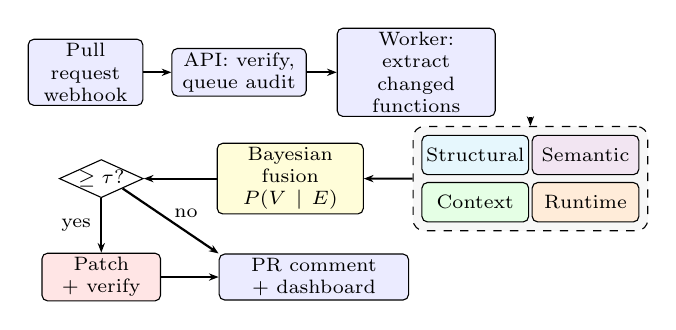
\begin{tikzpicture}[
  font=\scriptsize,
  box/.style={draw, rounded corners=2pt, align=center, minimum height=0.5cm,
              text width=#1, inner sep=1.5pt},
  box/.default=1.45cm,
  arr/.style={-{Stealth[length=3.5pt]}, thick}]
\node[box=1.35cm, fill=blue!8] (pr) at (0.4,0) {Pull request\\webhook};
\node[box=1.6cm, fill=blue!8] (api) at (2.35,0) {API: verify,\\queue audit};
\node[box=1.9cm, fill=blue!8] (ext) at (4.6,0) {Worker: extract\\changed functions};
\node[box=1.25cm, fill=cyan!10]   (s) at (5.35,-1.05) {Structural};
\node[box=1.25cm, fill=violet!10] (m) at (6.75,-1.05) {Semantic};
\node[box=1.25cm, fill=green!10]  (c) at (5.35,-1.65) {Context};
\node[box=1.25cm, fill=orange!15] (r) at (6.75,-1.65) {Runtime};
\begin{scope}[on background layer]
\node[draw, dashed, rounded corners, fill=gray!6, inner sep=3pt, fit=(s)(m)(c)(r)] (ag) {};
\end{scope}
\node[box=1.75cm, fill=yellow!15] (bay) at (3.0,-1.35) {Bayesian fusion\\$P(V\mid E)$};
\node[diamond, draw, aspect=2.2, inner sep=0pt, align=center] (dec) at (0.6,-1.35) {$\ge\tau$?};
\node[box=1.4cm, fill=red!10] (pat) at (0.6,-2.6) {Patch + verify};
\node[box=2.3cm, fill=blue!8] (out) at (3.3,-2.6) {PR comment\\+ dashboard};
\draw[arr] (pr) -- (api);
\draw[arr] (api) -- (ext);
\draw[arr] (ext.south -| ag.north) -- (ag.north);
\draw[arr] (ag.west) -- (bay.east);
\draw[arr] (bay) -- (dec);
\draw[arr] (dec) -- node[left]{yes} (pat);
\draw[arr] (pat) -- (out);
\draw[arr] (dec.south east) -- node[above right, inner sep=1pt]{no} (out.north west);
\end{tikzpicture}
\caption{Workflow of CodeSheriff. The four agents run blind.}
\label{fig:workflow}
\end{figure}

As illustrated in Fig.~\ref{fig:workflow}, the CodeSheriff workflow
consists of five stages:
\begin{enumerate}
\item \textbf{Trigger:} opening or updating a pull request sends a GitHub
webhook. The API verifies its HMAC-SHA256 signature, records an audit,
places it on a queue and replies within three seconds.
\item \textbf{Change Extraction:} a worker downloads the base and head
versions of each changed file and builds one unit per changed function.
\item \textbf{Agent Analysis:} the four agents analyse every unit
independently and produce structured evidence
(Algorithm~\ref{alg:agents}).
\item \textbf{Fusion and Decision:} the inference engine computes
$P(V\mid E)$ and the verdict, and alerted findings are passed to the patch
stage (Algorithm~\ref{alg:fusion}).
\item \textbf{Reporting:} one comment summarises the audit on the pull
request, and the verdict, probability, per-agent evidence and patch outcome
are stored for the dashboard.
\end{enumerate}

\subsection{Implementation}

CodeSheriff is a Python 3.12 monorepo. The API and the worker run as
separate processes with separate credentials: the API holds the webhook
secret, the worker holds the model key, and a queued task carries only an
audit identifier. Source code is held in memory only; the database stores
findings, evidence and hashes. The main components are:
\begin{itemize}
\item \textbf{Backend:} FastAPI with Celery and Redis for queued audits.
\item \textbf{Database:} PostgreSQL 16 with pgvector, SQLAlchemy, Alembic.
\item \textbf{Agents:} tree-sitter and a networkx taint engine with
Semgrep; a hosted LLM at $n=3$ samples; \texttt{bge-small-en-v1.5}
embeddings; Wasmtime with a WASI build of CPython.
\item \textbf{Dashboard:} Next.js with TypeScript and Recharts, read-only.
\item \textbf{Quality:} 1249 tests, strict type checking, and import rules
that stop any agent from importing another agent or the database.
\end{itemize}
\section{Experimental Evaluation}
\subsection{Environmental Setup}
We evaluate the prototype on a system with 16 GB RAM and an
Intel Core i5 processor. The implementation uses Python 3.12, Semgrep,
Tree-sitter, Sentence Transformers, pgvector, and a Wasmtime/WASI sandbox.
The system was evaluated based on calibration (expected calibration error,
Brier score) and detection accuracy (precision, recall, $F_1$).

\subsection{Comparative Analysis}
\label{subsec:comparison}

This subsection evaluates CodeSheriff's detection performance and
calibration quality against two classes of comparators: naive inference
baselines and external detectors evaluated on the same corpus, and related
systems reported in the literature. The goal is to establish not only
whether CodeSheriff detects vulnerabilities competitively, but whether its
reported confidence is trustworthy, a property largely unaddressed by
existing work, as discussed in Section~I.

Table~\ref{tab:comparison} reports CodeSheriff against inference baselines
and external detectors on the validation split ($n{=}15$ claims, 7
vulnerable), at the fitted alert threshold of $0.227$ and declared base
rate of $3\%$.

\begin{table}[t]
\centering
\caption{Detection and calibration on the validation split. Best per column
in bold.}
\label{tab:comparison}
\small
\setlength{\tabcolsep}{4pt}
\begin{tabular}{lccccc}
\toprule
System & ECE $\downarrow$ & Brier $\downarrow$ & P $\uparrow$ & R $\uparrow$ & $F_1$ $\uparrow$ \\
\midrule
Semgrep~\cite{semgrep}      & \missing{--} & \missing{--} & \missing{--} & \missing{--} & \missing{--} \\
Bandit~\cite{bandit}        & \missing{--} & \missing{--} & \missing{--} & \missing{--} & \missing{--} \\
Single LLM~\cite{ref17}     & \missing{--} & \missing{--} & \missing{--} & \missing{--} & \missing{--} \\
Prior only                  & \textbf{0.000} & 0.029 & 0.000 & 0.000 & 0.000 \\
Majority vote~\cite{ref16}  & 0.141 & \missing{--} & 0.076 & \textbf{1.000} & 0.142 \\
CodeSheriff (full)          & 0.027 & \textbf{0.013} & \textbf{1.000} & 0.857 & \textbf{0.923} \\
\bottomrule
\end{tabular}
\end{table}

CodeSheriff attains an $F_1$ of $0.923$ at perfect precision, alerting on 6
of 15 claims. Replacing Bayesian fusion with majority voting over the
identical evidence reduces $F_1$ to $0.142$ and raises ECE from $0.027$ to
$0.141$, since voting has no prior to moderate a single witness's alert. The
prior-only baseline reaches ECE $=0.000$ by detecting nothing, showing ECE
alone is insufficient; CodeSheriff's Brier score of $0.013$ (vs. $0.029$)
confirms it is calibrated \emph{and} decisive, not merely abstaining.

Beyond these internal baselines, Table~\ref{tab:related} positions
CodeSheriff against three related published systems.

\begin{table}[t]
\centering
\caption{Comparison with related systems. DeepSecure and Reddy et al. are
pending verification; MAVUL is not numerically comparable (different
language, CWE scope, and metric protocol).}
\label{tab:related}
\small
\setlength{\tabcolsep}{4pt}
\begin{tabular}{lcccc}
\toprule
Parameter & DeepSecure~\cite{ref2} & Reddy~\cite{ref6} & MAVUL~\cite{ref16} & Ours \\
\midrule
ECE $\downarrow$      & \missing{--} & \missing{--} & \missing{--} & 0.027 \\
Brier $\downarrow$    & \missing{--} & \missing{--} & \missing{--} & 0.013 \\
Precision $\uparrow$  & \missing{--} & \missing{--} & \missing{--} & 1.000 \\
Recall $\uparrow$     & \missing{--} & \missing{--} & \missing{--} & 0.857 \\
$F_1$ $\uparrow$       & \missing{--} & \missing{--} & \missing{--} & 0.923 \\
\bottomrule
\end{tabular}
\end{table}

DeepSecure is a Python-specific hybrid deep-learning detector with a
reported confidence component, and Reddy et al. is an agentic
vulnerability-triage system for collaborative software repositories; both
require verification of their reported metrics before their columns can be
populated. MAVUL, the closest multi-agent architectural precedent, is not
numerically comparable: it targets C/C++ memory-safety CWEs on a pairwise
dataset using its own P-C/P-V/P-B/P-R protocol rather than precision,
recall, or a calibration measure, and reports no reliability measure
alongside its detection results, consistent with the gap this paper
identifies in Section~I.

\subsection{Ablation Study}
\label{subsec:ablation}

This subsection isolates the contribution of each agent by removing it from
fusion and observing the effect on the posterior. Table~\ref{tab:ablation}
removes one witness at a time; a removed witness contributes an abstention
at likelihood ratio $1.0$, leaving the posterior unchanged except through
the evidence it no longer supplies.
\newline

\begin{table}[t]
\centering
\caption{Leave-one-witness-out ablation on the validation split at
threshold $0.227$. Best per column in bold.}
\label{tab:ablation}
\small
\setlength{\tabcolsep}{4pt}
\begin{tabular}{lccccc}
\toprule
Configuration & ECE $\downarrow$ & Brier $\downarrow$ & P $\uparrow$ & R $\uparrow$ & $F_1$ $\uparrow$ \\
\midrule
Full model     & 0.027 & \textbf{0.013} & \textbf{1.000} & \textbf{0.857} & \textbf{0.923} \\
\midrule
$-$ structural & \textbf{0.012} & 0.015 & \textbf{1.000} & 0.714 & 0.833 \\
$-$ semantic   & 0.047 & 0.031 & 0.096 & 0.429 & 0.157 \\
$-$ context    & 0.026 & \textbf{0.013} & \textbf{1.000} & \textbf{0.857} & \textbf{0.923} \\
$-$ runtime    & 0.028 & \textbf{0.013} & \textbf{1.000} & \textbf{0.857} & \textbf{0.923} \\
\bottomrule
\end{tabular}
\end{table}

The semantic witness dominates: its removal costs $0.766$ in $F_1$,
collapses precision to $0.096$, and is the only ablation that worsens
calibration (ECE $0.027 \rightarrow 0.047$). Removing the structural
witness costs $0.090$ in $F_1$ while improving ECE, the prior-only effect
in miniature: alerting less is easier to calibrate, not evidence for
removal. Context and runtime ablations leave the confusion matrix
unchanged on this split; both contribute measurably on the larger
calibration split, so this is reported as a null result, not redundancy.

\subsection{Assumptions and Limitations}
\label{subsec:limitations}

The reported results carry several caveats that bound their
generalizability. The corpus is Python-only, self-authored, and covers a
closed set of ten CWEs, so reported rates describe performance on this
corpus, not arbitrary pull requests. The validation split ($n{=}15$) is too
small to attach a meaningful interval to any figure in
Table~\ref{tab:comparison}, and the held-out test split remains unevaluated
at the time of writing. Evaluation is a single deterministic run against
committed model recordings, so no sampling variance is reported. The
structural witness ran with only one of its two backends available
(Semgrep lacks a build for the fitting platform), so its likelihood ratios
describe a one-backend witness. Finally, the $3\%$ base rate is declared,
not measured: the twin-paired corpus has a prevalence of $0.5$ by
construction, and every weighted figure inherits and rescales with this
assumption.

\section{Conclusion}
\label{sec:conclusion}

This paper presented CodeSheriff, a heterogeneous multi-agent security
auditor for GitHub pull requests that fuses structural, semantic,
contextual, and runtime evidence through Bayesian inference rather than
majority voting. On the validation split, CodeSheriff attained an $F_1$ of
$0.923$ at perfect precision with an expected calibration error of
$0.027$, outperforming a majority-vote combiner over the identical evidence
by a factor of $6.5$ in $F_1$ while more than halving calibration error.
The ablation study confirmed that this performance is not attributable to
any single agent: the semantic witness contributes the largest share of
detection power, while the structural, context, and runtime witnesses
contribute complementary, non-redundant evidence. Unlike existing
single-technique and multi-agent vulnerability detectors, which report a
verdict with no accompanying reliability measure, CodeSheriff's central
contribution is a posterior probability that is simultaneously
discriminative and calibrated, verified jointly through $F_1$ and Brier
score rather than either alone.

\section*{Future Work}
\label{sec:future}

Several items remain open from Section~\ref{subsec:limitations}. The
structural witness must be re-observed on a Linux or CI environment where
both backends, taint analysis and Semgrep, are available, since the
current fit describes a one-backend witness. The Semgrep, Bandit, and
single-LLM baselines require completion against the fitted artifact, and
the DeepSecure and Reddy et al. comparisons require verification of their
reported metrics before inclusion. The held-out test split remains
unevaluated and should be scored exactly once, per the evaluation protocol
in Section~\ref{sec:workflow}. Beyond the current evaluation, statistical
interval estimation and sensitivity analysis over the alert threshold and
declared base rate would strengthen confidence in the reported figures
given the small validation split. Finally, extending language coverage
beyond Python and evaluating a fine-tuned semantic model against the
current hosted-LLM configuration are both identified as future directions.

% \nocite{*}
\addcontentsline{toc}{section}{References}
\bibliographystyle{IEEEtran}
\bibliography{references}

\end{document}
